\documentclass[letterpaper,10pt,conference]{ieeeconf}
\IEEEoverridecommandlockouts
\overrideIEEEmargins
\usepackage[T1]{fontenc}
\usepackage[utf8]{inputenc}
\usepackage{lmodern}
\usepackage{amsmath,amssymb}
\usepackage{graphicx}
\usepackage{booktabs,array,tabularx}
\usepackage{cite}
\usepackage{url}
\usepackage{placeins}
\usepackage{tikz}
\usetikzlibrary{arrows.meta,positioning}
\usepackage[hidelinks]{hyperref}
\graphicspath{{figures/}}
\setlength{\emergencystretch}{2em}
\newcommand{\modelfigure}[3]{%
\begin{figure}[tb]\centering
\includegraphics[width=\columnwidth]{#1.pdf}
\caption{#2: held-out confusion matrix and ROC curve, using the common 261 observations. #3 AUC and the comparison metrics in Table~\ref{tab:comparison} are reported to three decimal places.}\label{fig:#1}
\end{figure}}
\title{\LARGE\bf Machine-Learning Prediction of Next-Quarter Stock-Price Direction in Indian and Non-Indian Biosimilar and Pharmaceutical Companies}
\author{Yuktha Ratna Puvvadi\\
{\small Birla Institute of Technology and Science, Pilani -- Hyderabad Campus}}
\begin{document}
\maketitle
\thispagestyle{plain}\pagestyle{plain}

\begin{abstract}
This study evaluates whether market and accounting features predict the next-quarter direction of stock prices in a pooled panel of Indian and non-Indian biosimilar and pharmaceutical companies. The reconstructed sample contains 3,375 retained company-quarters for 29 firms, with 2,911 training, 203 validation and 261 held-out test observations. Sixteen predictors enter eight classifiers after training-only imputation, clipping and standardisation. Financial reporting lags and purged partition boundaries constrain information availability. Fixed estimator specifications are compared using validation balanced accuracy; the support vector machine (SVM) is selected without test-driven tuning or refitting. Its test accuracy is 0.552, balanced accuracy is 0.551 and ROC-AUC is 0.520. The training-majority rule achieves test accuracy of 0.579; no classifier exceeds it in raw accuracy. Confusion matrices reveal materially different class trade-offs despite generally weak ranking performance. The results support a limited comparative finding for this historical panel, rather than evidence of a profitable forecasting strategy. Sparse accounting coverage and unverified historical data vintages constrain the interpretation.
\end{abstract}
\begin{keywords}
Stock-price direction, pharmaceutical companies, biosimilars, chronological evaluation, machine learning, class imbalance.
\end{keywords}

\section{Introduction and Research Problem}
The empirical question is whether information available at a company-quarter observation date can discriminate between a positive and a non-positive stock-price change over the following quarter. The sectoral universe comprises Indian and non-Indian biosimilar, biopharmaceutical and pharmaceutical companies. Sector membership defines the sample; the implemented predictors do not measure biosimilar product exposure, approvals or clinical events.

Direction prediction requires more than a high proportion of correct labels. When positive quarters predominate, a classifier can appear successful by frequently predicting an increase. A useful comparison must therefore evaluate both outcome classes, preserve the temporal order of observations and compare model performance with a simple rule fixed from training data. This paper addresses those requirements on one common reconstructed panel.

The contribution is a transparent comparison of eight fixed classifiers under a shared empirical design. The scope is deliberately bounded: a next-quarter price-direction task, pooled across firms, with model selection on an intermediate chronological partition. The analysis does not estimate causal financial relationships or implement a trading portfolio.

\section{Literature Review}
The methodological literature motivates contrasting model families rather than presuming that a more flexible classifier must forecast better. Random forests aggregate randomised decision trees~\cite{breiman2001}; gradient boosting constructs an additive model through successive loss-reducing fits~\cite{friedman2001}. These approaches accommodate nonlinear feature relationships in different ways. Support-vector networks use margin-based classification and nonlinear feature mappings~\cite{cortes1995}. Their relevance here is as alternative decision rules on the same observations, not as evidence of stock-market predictability.

The empirical comparison also includes a linear logistic classifier, a Gaussian conditional-density model, a multilayer perceptron, a local nearest-neighbour rule and a single decision tree. The implementation uses scikit-learn's common estimator interfaces~\cite{pedregosa2011}. A shared interface facilitates consistent preprocessing and evaluation but does not make the estimators' class weighting, capacity or optimisation identical.

ROC analysis separates score ranking from a particular classification threshold~\cite{fawcett2006}. This distinction matters when class prevalence and decision thresholds influence accuracy and sensitivity differently. Accordingly, this study combines confusion-derived measures with continuous-score ROC curves. These references establish methodological foundations; they do not establish sector-specific forecasting performance. The latter is tested only through the held-out results reported below.

\section{Research Objective and Defined Analytical Work}
The objective is to assess whether the available market and accounting features support out-of-period discrimination of next-quarter stock-price direction. The defined work consists of constructing company-quarter labels, applying explicit information lags, fitting common training transformations, comparing eight classifiers and interpreting held-out errors against the training-majority baseline. The model selected on validation balanced accuracy is evaluated without subsequent refitting. No new parameter search, threshold optimisation, regional model comparison or trading backtest is part of the completed experiment.

\section{Data and Empirical Design}
\subsection{Company Universe and Coverage}
The final reconstruction represents 15 Indian and 14 non-Indian companies. The Indian firms are Biocon, Aurobindo Pharma, Glenmark Pharmaceuticals, Sun Pharmaceutical, Torrent Pharmaceuticals, Alembic Pharmaceuticals, Natco Pharma, Ajanta Pharma, Marksans Pharma, Strides Pharma Science, Cipla, Jubilant Pharmova, Lupin, Zydus Lifesciences and Zenotech Laboratories. The non-Indian firms are Amgen, Biogen, Teva Pharmaceutical, Novartis, Fresenius SE, Merck \& Co., Baxter International, Viatris, Jiangsu Hengrui Pharma, Shanghai Fosun Pharma, Zhejiang Hisun Pharma, Pfizer, Sanofi and Formycon.

Laboratorios Rovi is excluded because the implemented daily-price input path supplies no usable daily CSV series for that company. This is a limitation of the reconstructed sample, not a statement about market-data availability in general. Zenotech contributes price observations despite missing accounting features under the implemented financial reader.

\subsection{Prices and Financial Statements}
Daily price observations retain local calendar dates. Invalid or non-positive prices are removed. The reconstruction uses adjusted close when available in the selected price block, otherwise close. It preserves the specified adjusted-series choices for Biocon, Ajanta Pharma, Marksans Pharma and Strides Pharma Science, and the Paris EUR series for Sanofi. Where selected inputs overlap, the longest valid source receives priority, with deterministic source ordering for ties.

Financial statement amounts are normalised from known reported units into base-currency amounts before ratios are constructed. No common-currency price-level predictor enters the model. The panel remains heterogeneous in listing history, reporting frequency and price-adjustment convention. These choices identify the implemented empirical sample; they do not establish a survivorship-free or point-in-time investment universe.

\section{Methodology}
Figure~\ref{fig:workflow} summarises the implemented analytical sequence.
\begin{figure}[!htbp]
\centering
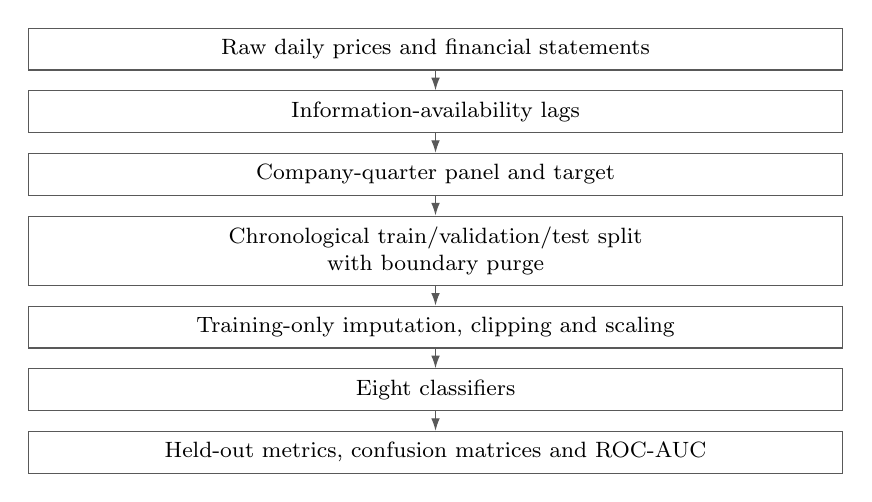
\begin{tikzpicture}[
  node distance=2.5mm,
  stage/.style={draw=black!65, line width=0.4pt,
    text width=0.83\columnwidth, align=center,
    inner xsep=4pt, inner ysep=4pt, font=\footnotesize},
  flow/.style={-{Latex[length=1.6mm,width=1.1mm]},
    draw=black!65, line width=0.45pt}
]
\node[stage] (raw) {Raw daily prices and financial statements};
\node[stage, below=of raw] (lags) {Information-availability lags};
\node[stage, below=of lags] (panel) {Company-quarter panel and target};
\node[stage, below=of panel] (split) {Chronological train/validation/test split\\with boundary purge};
\node[stage, below=of split] (preprocessing) {Training-only imputation, clipping and scaling};
\node[stage, below=of preprocessing] (models) {Eight classifiers};
\node[stage, below=of models] (evaluation) {Held-out metrics, confusion matrices and ROC-AUC};
\draw[flow] (raw) -- (lags);
\draw[flow] (lags) -- (panel);
\draw[flow] (panel) -- (split);
\draw[flow] (split) -- (preprocessing);
\draw[flow] (preprocessing) -- (models);
\draw[flow] (models) -- (evaluation);
\end{tikzpicture}
\caption{Implemented analytical workflow. Preprocessing is fitted on training observations and applied unchanged to validation and test data. Model selection uses validation balanced accuracy; held-out evaluation uses the saved decision rules.}
\label{fig:workflow}
\end{figure}

\subsection{Target Construction}
Let $P_{i,q}$ denote the latest valid observed price at or before calendar quarter-end $q$ for company $i$. Both the current and following quarter's endpoints must be no more than ten calendar days stale. Only observations with a following complete quarter are labelled. The realised return and binary target are
\begin{equation}
R_{i,q+1}=\frac{P_{i,q+1}}{P_{i,q}}-1,
\end{equation}
\begin{equation}
y_{i,q}=\begin{cases}1,&R_{i,q+1}>0,\\0,&R_{i,q+1}\leq0.\end{cases}
\end{equation}
Class 1 is ``up'' and class 0 is ``non-up'', including exactly zero returns. The outcome is price direction on the selected company-specific price basis. It is neither market-adjusted excess return nor an independently constructed total-return series.

\subsection{Feature Groups}
Sixteen predictors survive training-based feature screening: nine market measures and seven accounting measures. The market features are returns over 91, 182 and 365 calendar days; price-to-mean deviations over 20, 50 and 200 calendar days; daily-return sample standard deviations within 60- and 120-calendar-day windows; and volume change within 60 calendar days. Price-to-mean deviation is current price divided by the window mean minus one. Volume change compares mean volume in the later and earlier halves of the observations within the window. These are calendar windows, not fixed trading-session windows, and volatility is not annualised.

The accounting features are revenue growth, net profit margin, operating margin, return on equity, return on assets, current ratio and asset turnover. Revenue growth compares the nearest same-frequency period approximately one year earlier, allowing 45 days around that anniversary. Margins divide the corresponding income by revenue; return measures divide net income by ending equity or assets; current ratio divides current assets by current liabilities; asset turnover divides revenue by assets. Flow-to-stock measures use the selected reporting period, without annualisation or a trailing-twelve-month transformation.

Of 22 candidate definitions, debt-to-equity, price-to-book and the price-to-earnings proxy are entirely missing in training and are removed. Three further definitions are exact training duplicates: 3-month momentum of the 91-day return, 6-month momentum of the 182-day return, and the quick-ratio proxy of current ratio. Company identifiers and regional labels define observations but are not model predictors.

\subsection{Information Availability and Lag Rules}
Every market-feature calculation receives only prices dated on or before the observation quarter-end. Quarterly financial records become eligible at period-end plus 61 days; annual records at period-end plus 121 days. The latest eligible financial-period row must also be at most 200 days old for quarterly data or 550 days old for annual data. Missing fields in that row remain missing rather than being filled from arbitrarily old statements. Annual fallback can therefore change a financial ratio's horizon.

The lags implement an assumed release convention, not verified individual announcement dates. Revised statements and retrospectively adjusted prices may still differ from the information historically available to investors. Chronological feature rules reduce observable look-ahead but cannot establish historical vintage integrity.

\subsection{Chronological Train--Validation--Test Split}
Observation dates before 2022 enter the training partition, dates in 2022--2023 enter validation, and dates from 2024 enter test. A training label ending on or after 1 January 2022, or a validation label ending on or after 1 January 2024, is purged. This removes the 2021 Q4 and 2023 Q4 observation cohorts, totalling 58 company-quarters. The final split appears in Table~\ref{tab:split}. All classifiers use identical evaluation keys. The test labels extend through 2026 Q2 for the final 2026 Q1 observations.

\subsection{Training-Only Preprocessing}
Undefined and infinite numerical values are treated as missing. Feature retention and duplicate removal use training data only. Missing values are filled using training medians and clipped using the observed training 1st and 99th percentiles. A standard scaler is fitted after training imputation and clipping, then applied unchanged to validation and test observations. The same transformed 16-feature matrix enters every classifier. No synthetic observations or oversampling are used.

\subsection{Eight Classifiers and Selection Procedure}
Table~\ref{tab:specs} gives the fixed estimator settings. They are inherited specifications, not winners of a new hyperparameter search. Seeds are 42 wherever configured. Logistic regression, random forest, SVM and decision tree use balanced class weights; the other estimators do not. Thus the comparison includes both algorithm and class-treatment differences.
\begin{table*}[t]
\centering\small
\caption{Fixed classifier specifications. Balanced means inverse-frequency class weighting. No new hyperparameter search was performed.}\label{tab:specs}
\begin{tabularx}{\textwidth}{lXl}
\toprule
Classifier & Implemented settings & Class treatment \\
\midrule
Logistic Regression & L2 penalty; $C=1$; lbfgs; maximum 1000 iterations & Balanced \\
Random Forest & 100 trees; Gini; square-root feature sampling; unrestricted depth & Balanced \\
Naive Bayes & GaussianNB; variance smoothing $10^{-9}$; empirical priors & Unweighted \\
Gradient Boosting & 100 stages; learning rate 0.1; depth 3; log loss & Unweighted \\
SVM & RBF kernel; $C=1$; gamma=scale; probability estimation enabled & Balanced \\
Neural Network / MLP & One hidden layer of 100 ReLU units; Adam; $\alpha=0.0001$; learning rate 0.001; maximum 2000 iterations; early stopping disabled & Unweighted \\
K-Nearest Neighbours & Five neighbours; uniform voting; Minkowski distance with $p=2$ & Unweighted \\
Decision Tree & Gini; unrestricted depth; minimum one observation per leaf & Balanced \\
\bottomrule
\end{tabularx}
\end{table*}


The selection criterion is highest validation balanced accuracy, with validation ROC-AUC and then model name as deterministic tie-breakers. There is no refit on combined training and validation data. Predictions use each estimator's native decision rule: the binary SVM's decision boundary, and class argmax for the other estimators. The SVM's probability estimates are saved but do not replace its decision-function scores for ROC analysis. No test threshold is tuned. The MLP completed 779 iterations and logistic regression 12; the final training record contains no warnings.

\subsection{Classifier Formulations}
Let $\mathbf{x}\in\mathbb{R}^{p}$ denote the preprocessed feature vector, with $p=16$. The following formulations describe the fitted classifiers using the settings in Table~\ref{tab:specs} and the existing scikit-learn implementation~\cite{pedregosa2011}.

\paragraph{Logistic Regression}
The linear predictor is transformed into a positive-class probability:
\begin{equation}
\begin{aligned}
\Pr(y=1\mid\mathbf{x})&=\sigma(\beta_0+\mathbf{x}^{\top}\boldsymbol{\beta}),\\
\sigma(z)&=\frac{1}{1+e^{-z}}.
\end{aligned}
\end{equation}
The fitted coefficients use L2 regularisation and balanced class weights; classification follows the native binary decision rule.

\paragraph{Gaussian Naive Bayes}
Conditional feature independence gives
\begin{equation}
\Pr(y=c\mid\mathbf{x})\propto\Pr(y=c)
\prod_{j=1}^{p}\Pr(x_j\mid y=c).
\end{equation}
The implementation uses Gaussian class-conditional feature densities, empirical class priors and variance smoothing. Prediction selects the class with the largest posterior probability.

\paragraph{Random Forest}
The forest aggregates $B=100$ randomised trees~\cite{breiman2001}. Its implemented prediction averages tree class probabilities:
\begin{equation}
\hat{y}=\operatorname*{arg\,max}_{c\in\{0,1\}}
\frac{1}{B}\sum_{b=1}^{B}\hat{p}_b(c\mid\mathbf{x}).
\end{equation}
Here $\hat{p}_b$ is the class proportion in the reached leaf, accounting for training weights. This reduces to the modal tree label when all reached leaves assign probability one to a class; hard-label majority voting is not the general implemented rule.

\paragraph{Gradient Boosting}
The additive tree contribution is
\begin{equation}
F_M(\mathbf{x})=\sum_{m=1}^{M}\eta h_m(\mathbf{x}).
\end{equation}
The implementation uses $M=100$ stages, learning rate $\eta=0.1$ and depth-3 regression-tree weak learners, fitted sequentially under binary log loss~\cite{friedman2001}. Its positive-class probability is $\sigma(F_0+F_M(\mathbf{x}))$, where $F_0$ is the initial training-class log-odds. Retaining this intercept is necessary to describe the implemented score.

\paragraph{RBF Support Vector Machine}
For support vectors $SV$, the decision score is
\begin{equation}
\begin{aligned}
f(\mathbf{x})&=\sum_{i\in SV}\alpha_i y_i
\exp\!\left(-\gamma\|\mathbf{x}-\mathbf{x}_i\|^2\right)+b,\\
\hat{y}&=\mathbb{I}[f(\mathbf{x})>0].
\end{aligned}
\end{equation}
Within this expression, $y_i\in\{-1,+1\}$ is the signed encoding of the binary training label, and $\alpha_i$ are non-negative dual coefficients~\cite{cortes1995}. The fitted SVM uses $C=1$, $\gamma=\texttt{scale}$ and balanced class weights. ROC analysis uses $f(\mathbf{x})$, rather than the separately estimated probabilities.

\paragraph{Neural Network / MLP}
The binary network computes
\begin{equation}
\hat{p}(\mathbf{x})=\sigma\!\left(\mathbf{w}_2^{\top}
\operatorname{ReLU}(\mathbf{W}_1\mathbf{x}+\mathbf{b}_1)+b_2\right).
\end{equation}
It has one hidden layer of 100 ReLU units and uses Adam optimisation. The sigmoid output supplies the positive-class probability for the native classification rule.

\paragraph{K-Nearest Neighbours}
Uniform voting among the five nearest training observations gives
\begin{equation}
\hat{y}=\operatorname{mode}\{y_i:\mathbf{x}_i\in\mathcal{N}_5(\mathbf{x})\}.
\end{equation}
Neighbourhoods use Euclidean distance in the preprocessed feature space. All five neighbours have equal weight, and their positive-label fraction supplies the probability score.

\paragraph{Decision Tree}
Node impurity is measured by
\begin{equation}
G(t)=1-\sum_{c\in\{0,1\}}p_{c,t}^{2},
\end{equation}
where $p_{c,t}$ is the class-weighted proportion at node $t$. Among the candidate splits considered at each node, the chosen split minimises weighted child-node Gini impurity. Prediction selects the largest weighted class proportion in the reached leaf; the fitted tree uses balanced class weights and no depth cap.

These equations define the fixed evaluated specifications. They provide a compact account of the decision mechanisms, not an exhaustive derivation or a new hyperparameter search.

\subsection{Leakage Controls}
The completed verification found no duplicate company-quarter keys, future price-feature dates, assumed financial-availability violations, target-formula mismatches or split-label boundary violations. Independent checks reproduced saved metrics and model predictions. Future-price perturbation checks passed for all 29 represented companies. These checks validate the implemented timing and transformations; they do not validate historical financial publication vintages. The latter remains an explicit limitation.

\section{Evaluation Framework}
Confusion matrices use actual classes as rows and predicted classes as columns, ordered non-up then up. Consequently, their cells are $[TN,FP;FN,TP]$. Every classifier is evaluated on 151 positive and 110 non-positive test outcomes. The reported threshold-dependent measures are
\begin{equation}\text{Accuracy}=\frac{TP+TN}{TP+TN+FP+FN},\end{equation}
\begin{equation}\text{Precision}=\frac{TP}{TP+FP},\end{equation}
\begin{equation}\text{Sensitivity}=\frac{TP}{TP+FN},\end{equation}
\begin{equation}\text{Specificity}=\frac{TN}{TN+FP},\end{equation}
\begin{equation}F_1=\frac{2TP}{2TP+FP+FN},\end{equation}
\begin{equation}\text{Balanced Accuracy}=\frac{\text{Sensitivity}+\text{Specificity}}{2}.\end{equation}
Recall and sensitivity denote the same positive-class measure. The implementation assigns zero to undefined precision, recall or F1; denominators for the reported eight-model test results are nonzero.

The ROC curve plots sensitivity against false-positive rate across score thresholds. ROC-AUC measures threshold-independent ranking: the probability that a randomly chosen positive outcome receives a higher score than a randomly chosen negative outcome, with half credit for tied scores~\cite{fawcett2006}. It is not the fraction of correct labels at the saved decision rule, nor proof of probability calibration. All eight test sets contain both classes, so their AUC values are valid. Scores are positive-class probabilities except for SVM, which uses the positive-class decision function.

The baseline always predicts the training-majority class, up, because training contains 1,726 positive and 1,185 non-positive outcomes. Its constant score is the training positive fraction. It is fixed before evaluation and has ROC-AUC and balanced accuracy of 0.500. No uncertainty intervals, significance tests or transaction-cost evaluation were produced; conclusions below are descriptive.

\section{Results}
\subsection{Sample and Split}
The reconstructed panel contains 3,433 labelled company-quarters before the boundary purge and 3,375 retained observations after it. Training is historically unbalanced, beginning in 1962 for the longest series and expanding with company coverage. Validation and test each contain all 29 firms in every retained quarter. This is not a balanced panel covering only recent years.
\begin{table*}[t]
\centering\small
\caption{Retained chronological partitions. Dates refer to observation quarter-ends, not outcome quarter-ends. Each partition represents 29 companies; early training coverage is unbalanced.}\label{tab:split}
\begin{tabular}{lrrrrll}
\toprule
Partition & Observations & Up & Non-up & Companies & First observation & Last observation \\
\midrule
Training & 2911 & 1726 & 1185 & 29 & 1962-03-31 & 2021-09-30 \\
Validation & 203 & 117 & 86 & 29 & 2022-03-31 & 2023-09-30 \\
Test & 261 & 151 & 110 & 29 & 2024-03-31 & 2026-03-31 \\
\bottomrule
\end{tabular}
\end{table*}

\begin{figure}[tb]\centering
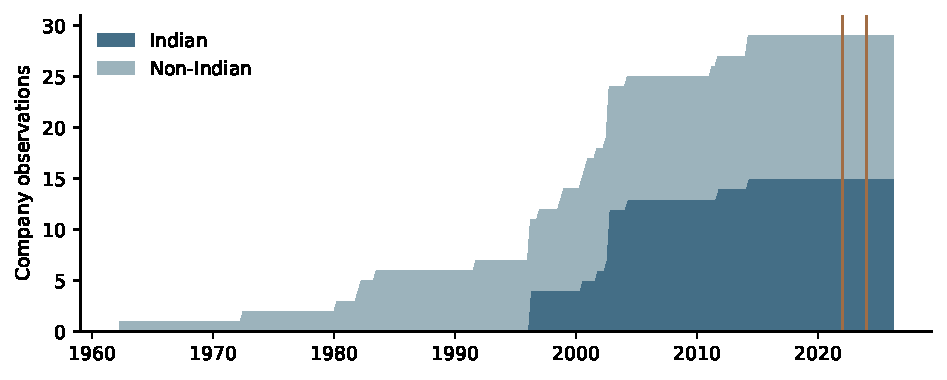
\includegraphics[width=\columnwidth]{coverage.pdf}
\caption{Retained company-quarter coverage by region. Vertical markers identify the 2022 and 2024 observation-date boundaries. Early history is uneven; the two boundary observation cohorts are purged.}\label{fig:coverage}
\end{figure}

\subsection{Full Model Comparison}
Table~\ref{tab:comparison} reports all test metrics to three decimal places, with confusion counts in Table~\ref{tab:confusion}. Abbreviations are LR (logistic regression), RF (random forest), NB (Naive Bayes), GB (gradient boosting), SVM, MLP (neural network), KNN and DT (decision tree). The baseline is shown alongside the classifiers. Figure~\ref{fig:comparison} compares accuracy, balanced accuracy and ranking performance; Figure~\ref{fig:roc} shows all continuous-score ROC curves.
\begin{table*}[t]
\centering\footnotesize
\caption{Complete held-out model comparison ($n=261$). Metrics are reported to three decimal places. Recall is sensitivity. Both panels refer to the same fitted models and predictions.}\label{tab:comparison}
\setlength{\tabcolsep}{6pt}
\begin{tabular}{lrrrr}
\toprule
Model & Accuracy & Precision & Recall / sensitivity & Specificity \\
\midrule
LR & 0.494 & 0.573 & 0.497 & 0.491 \\
RF & 0.533 & 0.581 & 0.689 & 0.318 \\
NB & 0.425 & 0.510 & 0.166 & 0.782 \\
GB & 0.510 & 0.561 & 0.695 & 0.255 \\
SVM & 0.552 & 0.627 & 0.556 & 0.545 \\
MLP & 0.487 & 0.555 & 0.570 & 0.373 \\
KNN & 0.467 & 0.537 & 0.576 & 0.318 \\
DT & 0.487 & 0.553 & 0.583 & 0.355 \\
Baseline & 0.579 & 0.579 & 1.000 & 0.000 \\
\bottomrule
\end{tabular}
\par\medskip
\begin{tabular}{lrrrr}
\toprule
Model & F1-score & Balanced accuracy & ROC-AUC & Predicted up fraction \\
\midrule
LR & 0.532 & 0.494 & 0.514 & 0.502 \\
RF & 0.630 & 0.503 & 0.477 & 0.686 \\
NB & 0.250 & 0.474 & 0.503 & 0.188 \\
GB & 0.621 & 0.475 & 0.491 & 0.716 \\
SVM & 0.589 & 0.551 & 0.520 & 0.513 \\
MLP & 0.562 & 0.471 & 0.466 & 0.594 \\
KNN & 0.556 & 0.447 & 0.460 & 0.621 \\
DT & 0.568 & 0.469 & 0.469 & 0.609 \\
Baseline & 0.733 & 0.500 & 0.500 & 1.000 \\
\bottomrule
\end{tabular}
\end{table*}

\begin{table}[tb]
\centering\small
\caption{Held-out confusion counts. All models share 110 non-up and 151 up outcomes.}\label{tab:confusion}
\begin{tabular}{lrrrr}
\toprule
Model & TN & FP & FN & TP \\
\midrule
LR & 54 & 56 & 76 & 75 \\
RF & 35 & 75 & 47 & 104 \\
NB & 86 & 24 & 126 & 25 \\
GB & 28 & 82 & 46 & 105 \\
SVM & 60 & 50 & 67 & 84 \\
MLP & 41 & 69 & 65 & 86 \\
KNN & 35 & 75 & 64 & 87 \\
DT & 39 & 71 & 63 & 88 \\
Baseline & 0 & 110 & 0 & 151 \\
\bottomrule
\end{tabular}
\end{table}

\begin{figure*}[t]\centering
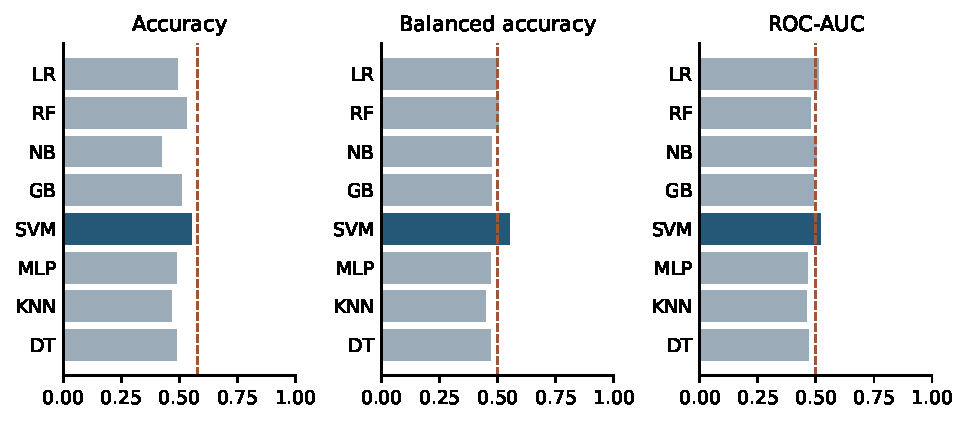
\includegraphics[width=0.88\textwidth]{comparison.pdf}
\caption{Held-out classifier comparison. Dashed lines indicate majority-baseline accuracy in the first panel and 0.500 in the balanced-accuracy and ROC-AUC panels. The SVM is highlighted because validation selected it.}\label{fig:comparison}
\end{figure*}
\begin{figure*}[t]\centering
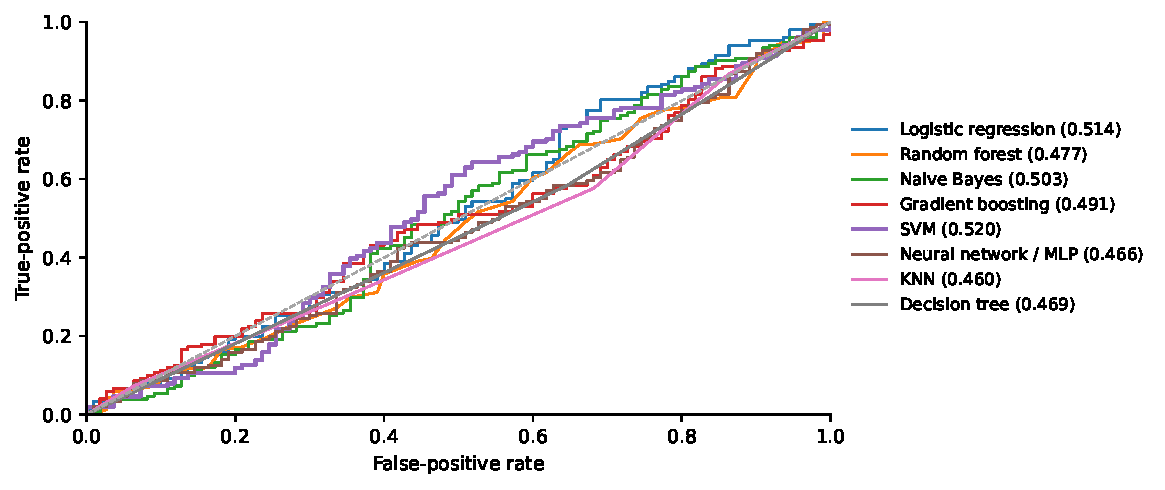
\includegraphics[width=0.88\textwidth]{roc_comparison.pdf}
\caption{Held-out ROC curves for all eight classifiers. Scores are positive-class probabilities except for SVM decision-function scores. AUC values are shown to three decimal places, as in Table~\ref{tab:comparison}.}\label{fig:roc}
\end{figure*}

\subsection{Individual Model Results}
\paragraph{Logistic Regression}
The linear model correctly classifies 54 non-up and 75 up quarters, while missing 76 up outcomes. Its sensitivity and specificity are both below 0.500 at the native decision rule. AUC is slightly above 0.500, indicating that the ranking and the thresholded classification need not give the same assessment (Fig.~\ref{fig:logistic_regression}).
\modelfigure{logistic_regression}{Logistic regression}{ROC uses positive-class probabilities.}

\paragraph{Random Forest}
The forest detects 104 positive outcomes but predicts up for 75 of the 110 non-up quarters. Its positive-class F1 is the largest among the eight fitted classifiers, yet its AUC is below 0.500 and balanced accuracy only slightly exceeds 0.500. The confusion matrix shows why a comparatively high F1 does not establish useful discrimination across both classes (Fig.~\ref{fig:random_forest}).
\modelfigure{random_forest}{Random forest}{ROC uses positive-class probabilities.}

\paragraph{Naive Bayes}
Gaussian Naive Bayes correctly identifies 86 non-up quarters, the largest true-negative count among the fitted classifiers, but detects only 25 up quarters. Its 126 false negatives account for its low sensitivity and F1. Its near-chance AUC shows that high specificity at this decision rule does not imply strong overall ranking (Fig.~\ref{fig:naive_bayes}).
\modelfigure{naive_bayes}{Naive Bayes}{ROC uses positive-class probabilities.}

\paragraph{Gradient Boosting}
Boosting has 105 true positives, the largest count among the eight classifiers, but also 82 false positives. The resulting sensitivity advantage is accompanied by low specificity and balanced accuracy below 0.500. The ROC curve does not provide evidence that this trade-off conceals strong ranking performance (Fig.~\ref{fig:gradient_boosting}).
\modelfigure{gradient_boosting}{Gradient boosting}{ROC uses positive-class probabilities.}

\paragraph{Support Vector Machine}
SVM correctly identifies 60 non-up and 84 up quarters, with 50 false positives and 67 false negatives. Its test sensitivity of 0.556 and specificity of 0.545 are comparatively even. It has the highest test accuracy, balanced accuracy and AUC among the eight fitted classifiers, although selection occurred on validation data. The weak AUC of 0.520 limits the substantive claim (Fig.~\ref{fig:svm}).
\modelfigure{svm}{Support vector machine}{ROC uses decision-function scores; the marker denotes the native decision boundary, not a probability threshold of 0.500.}

\paragraph{Neural Network / MLP}
The MLP identifies 86 positive and 41 non-positive outcomes. Its 69 false positives and 65 false negatives yield accuracy below 0.500, and its AUC is also below 0.500. The completed fit produced no convergence warning, so the result should be reported as the outcome of this fixed specification rather than dismissed as an unfinished optimisation (Fig.~\ref{fig:neural_network}).
\modelfigure{neural_network}{Neural network / MLP}{ROC uses positive-class probabilities.}

\paragraph{K-Nearest Neighbours}
KNN yields 87 true positives and 35 true negatives. It has the lowest test balanced accuracy and ROC-AUC among the eight classifiers. The proximity structure induced by the shared scaled features therefore does not produce effective discrimination under the fixed five-neighbour rule (Fig.~\ref{fig:knn}).
\modelfigure{knn}{K-nearest neighbours}{ROC uses positive-class vote proportions.}

\paragraph{Decision Tree}
The single tree identifies 88 positive and 39 non-positive outcomes. Its test accuracy equals the MLP's, although their error distributions differ. The saved tree scores produce a coarse ROC curve; AUC and balanced accuracy agree up to floating-point representation. This is a property of the saved predictions, not a general equivalence between these metrics (Fig.~\ref{fig:decision_tree}).
\modelfigure{decision_tree}{Decision tree}{ROC uses positive-class leaf probabilities.}

\subsection{Baseline Comparison and Model Selection}
The baseline correctly labels all 151 up quarters and none of the 110 non-up quarters. Its accuracy, 0.579, exceeds every fitted classifier, including the selected SVM at 0.552. In counts, SVM makes 144 correct predictions versus the baseline's 151: detecting 60 non-up quarters does not offset its 67 missed up quarters in raw accuracy. SVM does outperform the baseline's 0.500 balanced accuracy, because it recognises both classes.

Table~\ref{tab:validation} documents the validation selection comparison. SVM leads validation balanced accuracy at 0.535, with validation AUC of 0.578. Its selection is justified by that stated criterion, not by beating the majority rule in accuracy or by demonstrated economic value. Figure~\ref{fig:tradeoffs} shows the class trade-offs behind the aggregate metrics.
\begin{table}[tb]
\centering\footnotesize
\caption{Validation selection metrics ($n=203$), shown to three decimal places. SVM maximises balanced accuracy.}\label{tab:validation}
\setlength{\tabcolsep}{3pt}
\begin{tabular}{lrr}
\toprule
Model & Balanced accuracy & ROC-AUC \\
\midrule
LR & 0.486 & 0.541 \\
RF & 0.509 & 0.487 \\
NB & 0.515 & 0.478 \\
GB & 0.463 & 0.492 \\
SVM & 0.535 & 0.578 \\
MLP & 0.516 & 0.531 \\
KNN & 0.487 & 0.481 \\
DT & 0.489 & 0.489 \\
Baseline & 0.500 & 0.500 \\
\bottomrule
\end{tabular}
\end{table}

\begin{figure}[tb]\centering
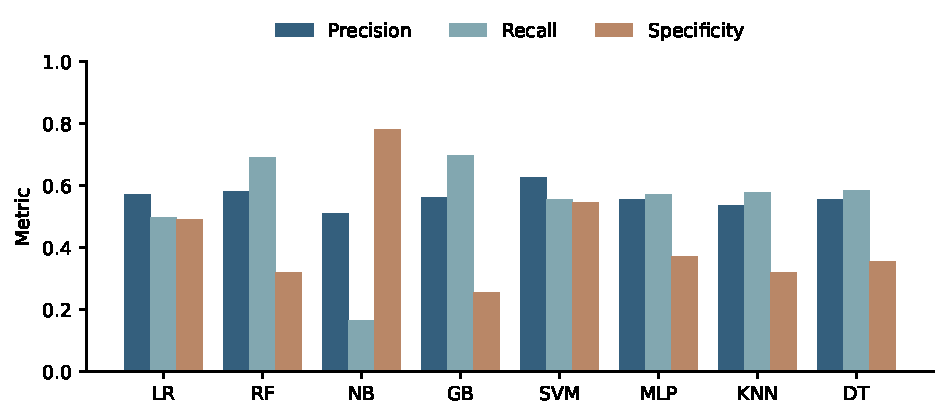
\includegraphics[width=\columnwidth]{class_tradeoffs.pdf}
\caption{Held-out precision, sensitivity (labelled recall) and specificity. NB favours non-up recognition, whereas RF and GB favour up recognition. The SVM's sensitivity and specificity are more even.}\label{fig:tradeoffs}
\end{figure}

\subsection{Feature and Model Diagnostics}
Accounting information is substantially sparser than price information, especially in training (Fig.~\ref{fig:missingness}). Median imputation therefore makes a large part of the early accounting feature matrix constant. The change in missingness between historical training and recent evaluation partitions is itself a limitation on comparability.
\begin{figure}[tb]\centering
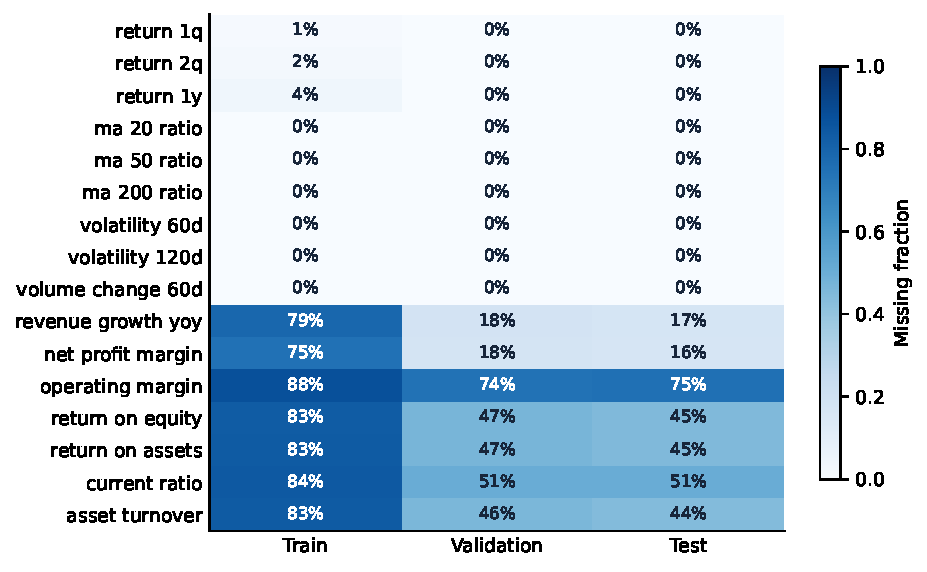
\includegraphics[width=\columnwidth]{missingness.pdf}
\caption{Missing fractions before imputation for all 16 retained features, by split. Percentage labels retain the original display rounding. Accounting coverage is much weaker than market-feature coverage.}\label{fig:missingness}
\end{figure}

The largest positive logistic coefficient belongs to the 182-day return and the largest negative coefficient to the 50-day price-to-mean deviation (Fig.~\ref{fig:coefficients}). These are conditional associations after training clipping and scaling; correlated inputs, class weighting and imputation preclude a causal interpretation.
\begin{figure}[tb]\centering
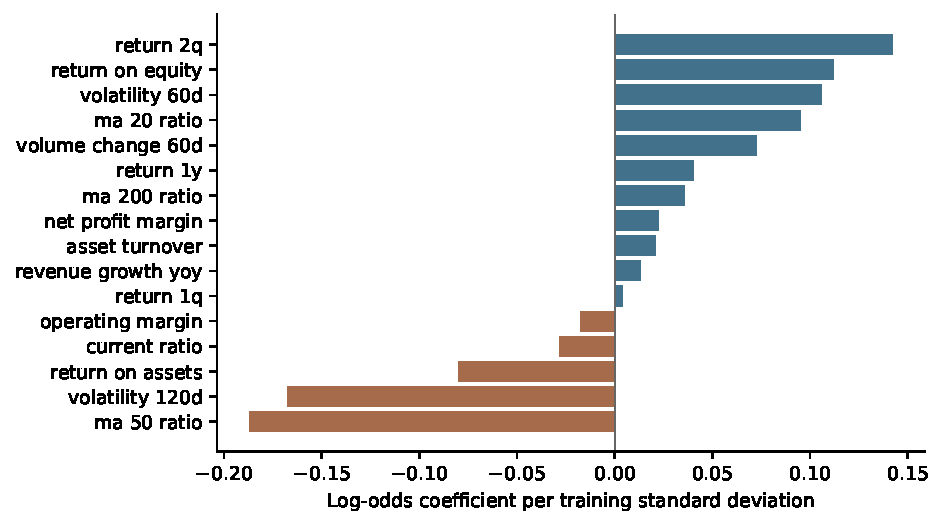
\includegraphics[width=\columnwidth]{logistic_coefficients.pdf}
\caption{Logistic coefficients per training standard deviation of the transformed features. Signs describe fitted conditional associations with the up class, not causal price effects.}\label{fig:coefficients}
\end{figure}

SVM permutation importance uses validation balanced accuracy and ten repeats (Fig.~\ref{fig:importance}). Revenue growth has the largest positive mean decrease, followed by asset turnover and the 182-day return. Several mean decreases are negative and variability is substantial. These diagnostics do not establish robust financial drivers and were not used to reselect features using test data.
\begin{figure}[tb]\centering
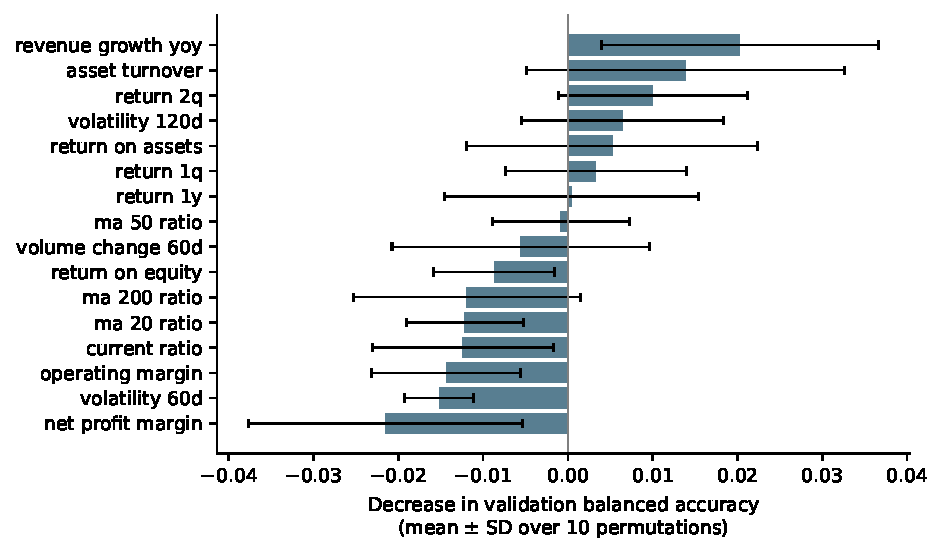
\includegraphics[width=\columnwidth]{selected_importance.pdf}
\caption{Selected SVM: mean decrease in validation balanced accuracy after feature permutation. Error bars are standard deviations across ten permutations, not confidence intervals. Negative values mean that permutation improved the measured score on average.}\label{fig:importance}
\end{figure}
\FloatBarrier

\section{Discussion}
The principal result is the divergence between majority-class accuracy and two-class discrimination. SVM provides the best balance among these fixed classifiers, but it does not improve raw accuracy over always predicting an increase. RF and GB detect more up quarters while accepting many false positives; NB recognises more non-up quarters while missing most positive outcomes. No single metric adequately describes these patterns.

The ROC results further temper the threshold-based comparisons. Even the highest held-out AUC is close to 0.500, and the selected model's validation ranking performance does not persist at the same level in test. It would therefore be misleading to present validation selection as evidence of a strong or deployable forecasting advantage. Positive-class F1 also favours frequent up predictions and must be interpreted alongside specificity and the baseline.

The historical panel supplies many price observations but does not supply equally rich contemporaneous fundamentals. Mixing long listing histories with sparse early accounting coverage can make the effective information set differ sharply across time. The current experiment cannot isolate the contributions of accounting data, historical window length or region because it contains no feature ablation, rolling-window comparison or separate regional evaluation. The feature diagnostics suggest questions for those studies, not answers to them.

\section{Limitations}
The test set contains only nine observation quarters, with 29 firms exposed to potentially shared market conditions. Company-quarters should not be assumed statistically independent. No cluster-aware uncertainty estimates or repeated chronological evaluations are available, so small metric differences cannot be called statistically significant.

The selected company universe is retrospective and the training panel highly unbalanced. Survivorship, listing changes and structural shifts are not controlled through historical membership reconstruction. The company histories span very different market environments, and the fixed training window does not test whether recent observations would generalise better.

Financial eligibility uses assumed lags and age limits rather than verified release timestamps. Point-in-time statement vintages and adjustment histories are unverified. Annual and quarterly accounting rows yield different flow horizons, and heavy median imputation can suppress variation. These limitations remain despite successful mechanical timing checks.

The eight specifications have unequal class weighting and no systematic tuning budget. Their comparison therefore supports conclusions about the fitted configurations, not a universal ranking of algorithm families. No probability-calibration assessment, event-specific predictors, return-magnitude modelling, trading costs, portfolio construction or risk-adjusted performance was evaluated. Price-direction accuracy alone cannot establish investment usefulness.

\section{Conclusion}
A common chronology and training-only preprocessing make the eight classifiers comparable on 261 held-out company-quarters. Validation selects SVM, whose test balanced accuracy exceeds the majority rule's 0.500, but whose raw accuracy remains below that rule. None of the eight classifiers beats the majority-class baseline in test accuracy, and their ROC results indicate limited ranking performance. The defensible conclusion is modest two-class discrimination for the selected configuration within this reconstructed panel, with no demonstrated trading advantage. Further work requires historically available financial vintages, more complete features and repeated chronological evaluation before stronger predictive claims can be assessed.

\bibliographystyle{IEEEtran}
\bibliography{references}
\end{document}
